\documentclass{article}
\usepackage[a6paper,
            total={105mm, 148mm},
            margin=30pt,
            twoside % Tillåter olika placering av sidnummer på udda och jämna sidor
]{geometry}
\usepackage{fancyhdr}
\usepackage{parselines}
\usepackage{float}
\usepackage{graphicx}
\usepackage[absolute,overlay]{textpos}  % Package for absolute positioning
\usepackage{atbegshi}

\usepackage{imakeidx} % Registret
\usepackage{background} % Gråa Krusidull-E:et och alla bilder
\usepackage{ifoddpage} % Gråa Krudidull-E:et på udda sidor


\usepackage{xcolor} % BARA I BÖRJAN FÖR MARKERING TILL OSS SJÄLVA


% Normal background setup for odd pages
\backgroundsetup{
  scale=0.65,
  opacity=0.075,
  angle=0,
  color=black,
  vshift=-130,
  hshift=50,
  contents={%
    \checkoddpage
    \ifoddpage
      
\includegraphics[width=\paperwidth]{./bilder/large_E.png}
    \else
      %
\includegraphics[width=\paperwidth]{../bilder/VarumarkesBildServlet.jpg}
    \fi
  }
}


\newcommand{\custombackground}[1]{
  \backgroundsetup{
    scale=0.65,
    opacity=0.0,
    angle=0,
    color=black,
    vshift=-130,
    hshift=50,
    contents={\includegraphics[width=\paperwidth]{#1}}
  }
}

\newcommand{\noBackground}{
  \backgroundsetup{
    scale=0.65,
    opacity=0.0,
    angle=0,
    color=black,
    vshift=-130,
    hshift=50,
    contents={
\includegraphics[width=\paperwidth]{./bilder/no_background.png}}
  }
}


\newcommand{\resetBackground}{
  \backgroundsetup{
    scale=0.65,
    opacity=0.075,
    angle=0,
    color=black,
    vshift=-130,
    hshift=50,
    contents={%
      \checkoddpage
      \ifoddpage
        
\includegraphics[width=\paperwidth]{./bilder/large_E.png}
      \else
        %
\includegraphics[width=\paperwidth]{../bilder/VarumarkesBildServlet.jpg}
      \fi
    }
  }
}



% Disable indentation for the whole document
\setlength{\parindent}{0pt}


% Use fontspec with XeLaTeX or LuaLaTeX to load system fonts
\usepackage{fontspec}

% Set up the subsection font to Lucida Sans Unicode
\usepackage{titlesec}
\titleformat{\subsection}
  {\normalfont\fontsize{12pt}{10pt}\selectfont\fontspec{Lucida Sans Unicode}} % Adjust the size if needed
  {\thesubsection}{1em}{}

% Adjust vertical spacing around subsection titles
\titlespacing{\subsection}
{0pt}                % Left margin
{0.5ex plus .2ex}    % Space before subsection title (adjust as needed)
{0.5ex plus .2ex}    % Space after subsection title (adjust to decrease space after)

% Adjust footskip to add space below the footer
% \setlength{\footskip}{20pt} % Flyttar upp footern lite ########################################## Denna funkar inte riktigt som jag trodde. Jag vill flytta upp sidnumret lite mer
\setlength{\textheight}{120mm}


% Define the page style
\fancypagestyle{main}{
  \fancyhf{} % clear all header and footer fields
  \fancyhead[RO]{\hfill \footnotesize\scshape\leftmark \hfill}
  % \fancyfoot[LE,RO]{\thepage}

  % Adjust the page number position
  % Set page number closer to the edge by increasing the right margin
  \fancyfoot[LE]{\hspace{-17pt}\thepage} % Flytta ut sidnummer jämna sidor
  \fancyfoot[RO]{\thepage\hspace{-17pt}} % Flytta ut sidnummer udda sidor

  % Ta bort linje under/över header och footer
  \renewcommand{\headrulewidth}{0 pt}
  \renewcommand{\footrulewidth}{0 pt}

  % Använder footnote for 'visste du att'
  \renewcommand{\footnoterule}{}
  \renewcommand{\thefootnote}{}
}

% Set up textblock package to work with A6 paper
\setlength{\TPHorizModule}{1mm}  % Set horizontal units to mm
\setlength{\TPVertModule}{1mm}   % Set vertical units to mm

% Define the custom command to place text at the bottom of the page
\newcommand{\vissteduatt}[1]{%
    \begin{textblock*}{100mm}(12mm,137mm) % Adjust (2.5mm, 140mm) to position text
        \raggedright
        {\footnotesize{\textit{#1}}}
    \end{textblock*}
    \newpage % Ensures that the text appears only on the current page
}


% Define the custom command for small font and italics
\newcommand{\songinfo}[1]{%
  \textit{\small #1 \\}%
}









% DETTA SÄTTET ATT GÖRA REGISTER FUNGERAR BRA OCH ÄR LÄTT MEN DET BLIR INTE LIKA SNYGGT UTAN PUNKTERNA



% HITTA ETT SÄTT ATT GÖRA ETT SNYGGARE REGISTER INNAN VI FORTSÄTTER ATT LÄGGA TILL LÅTAR ETC. 
\makeindex[ % Alfabetiskt register
  name=alfa,
  columns=1,
  title=Alfabetiskt Register,
  intoc,
  options = {-s styleAlfa.ist}
]
\makeindex[ % Analfabetiskt register -- början av sången
  name=anfa,
  columns=1,
  title=Analfabetiskt Register,
  intoc,
  options = {-s styleAlfa.ist}
]


\begin{document}

% Apply the 'main' page style
\pagestyle{main}

% Title and empty page without header/footer
\NoBgThispage
\begin{titlepage}
    \centering
    \vspace{1cm}
    {\fontsize{18}{18}\selectfont E-sektionens sångbok}\\
    \vspace{0.2cm}
    {\fontsize{30}{30}\textbf{Komponenten}}\\
    \vspace{0.2cm}
    {\fontsize{15}{15}\textit{2:a upplagan}}
    \thispagestyle{empty}

    \begin{figure}[H]
      \centering
      
\includegraphics[width=1\textwidth]{./bilder/large_E.png}
    \end{figure}

\end{titlepage}


\newpage


Borra ett hål i pärmen här för att fästa din penna: {\Huge $\bullet$}

\subsubsection*{Konsten att sjunga!}
Att sjunga är verkligen något av det roligaste som finns\dots


Jag vet inte riktigt vad vi vill skriva här\dots

Att sjunga är kul\dots



Morris Thånell BME19 och Elin Helmersson E21\\
Sångbokskommittén 2024



\newpage

Tack till de som hjälpt oss med boken!

\newpage

\begin{center}
    \textbf{Viktig information}
\end{center}

% \backgroundsetup{ 
%   scale=0.36,
%   opacity=1,
%   angle=0,
%   color=black,
%   vshift=300,
%   hshift=151,
%   contents={
\includegraphics[width=\paperwidth]{./bilder/profilbild.png}}
% }

\begin{textblock*}{6cm}(6cm,1.5cm) % {block width}(x-coordinate, y-coordinate)
  
\includegraphics[width=3.5cm]{./bilder/profilbild_stor.png} % Adjust the image size as needed
\end{textblock*}
\begin{parse lines}[\noindent]{#1\\}
    Ägare:

    Sektion(?):
    
    Inskrivningsår:
    
    Födelsedatum:



    Lämna tillbaka mig till den här adressen:


    Hittelön:
    Om jag inte varit teknolog hade jag varit:
    Om jag fick välja nollningstema:


    Favoritmat:
    Favoritband:
    Favorit
    Bästa 
    Favoritintegral:
    
    .... Rita eller klistra en bild

\end{parse lines}

\newpage

% \subsubsection*{Innehållsförteckning}
\tableofcontents

\newpage
\begin{center}
  \vspace*{1.5cm}
  {\fontsize{20}{20}\textbf{Vett och etikett}}\\
  \vspace{0.7cm}
  {\fontsize{12}{12}\textit{Om den pryde själv får välja}}
\end{center}
\addtocwithheader{Vett och etikett}  % Add entry to TOC and set header
\noBackground
\newpage

\subsubsection*{KLÄDKOD}
För att underlätta förmedlingen av vem som ska ha på sig vad använder vi oss av följande namn.

\textbf{Truls}: Manlig teknolog\\
\textbf{Trula}: Kvinnlig teknolog\\
\textbf{Trelsa}: För hen som inte vill identifiera sig med någon av ovanstående.\\

\subsubsection*{Högtidsdräkt - Militäruniform och folkdräkt}

\textbf{Truls}: Militäruniform, folkdräkt eller frack\\
\textbf{Trula}: Militäruniform, folkdräkt eller balklädding\\
\textbf{Trelsa}: Se Truls/Trula\\

\subsubsection*{Civil högtidsdräkt}

\textbf{Truls}: Frack, vit skjorta, vit fluga\\
\textbf{Trula}: Balklädding\\
\textbf{Trelsa}: Se Truls/Trula\\

\subsubsection*{Smoking}
\textbf{Truls}: Smoking, vit skjorta, svart fluga\\
\textbf{Trula}: Lång klänning, dock behöver den inte vara lika elegant som en Balklädding. Tänk festligt.
\textbf{Trelsa}: Se Truls/Trula\\

\subsubsection*{Mörk kostym}
\textbf{Truls}: Mörkblå, mörkgrå eller svart kostym. Vit skjorta med sidenslips eller fluga i valfri färg.\\
\textbf{Trula}: En finare känning, men även byxdress elelr halvlång kjol med jacka går bra.\\
\textbf{Trelsa}: Se Truls/Trula\\

\subsubsection*{Kavaj}
Ibland även kallad bruten elelr udda kavaj.\\
\textbf{Truls}: Kavaj och ett par finare byxor (dock inte kostymbyxor), skjorta i valfri färg. Fluga eller slips kan vara trevligt!\\
\textbf{Trula}: Cocktailklänning, kjol eller dress.\\
\textbf{Trelsa}: Se Truls/Trula\\

\subsubsection*{Mörk kostym}
\textbf{Truls}: Ouvve \textbf{Hur vill vi stava ouvve/ovve i boken?}\\
\textbf{Trula}: Ouvve\\
\textbf{Trelsa}: Se Truls/Trula\\


\subsubsection*{KLÄDKOD version 2?}
Kåren har ett annat upplägg på hur de visar klädkoderna. Vill vi göra som dem?
\\

Exempel (kopierat från kårens bok)

\subsubsection*{Högtidsdräkt/högtidsklädsel}
För honom är frack lämplig. 
En fin golvlång klänning gäller för henne 
- ett bra material och ett tjusigt sntit ska det vara på den. 
Vill man bära handskar till klänningen går det bra, 
men glöm inte att ta av dem när du äter. 
Både han och hon kan istälet bära hembygdsdräkt eller militär högtidsdräkt.


\newpage

\subsubsection*{ETIKETT}

\subsubsection*{Vid bordet}
Han har sin bordsdam till höger om sig och hon har sin bordsherre till vänster.
Herren drar ut stolen till höger för att hjälpa sin bordsdam till bords eller från bordet. 


\textbf{Denna visste du att måste nog skrivas om eller ändra storleken på all text i boken. Vi ahr lite större text än i gamla komponenten vilket göra att vi inte får plats med riktigt lika mycket text på varje sida....}

\vissteduatt{Visste du att bordsherre och bordsdam är bordsplaceringsbenämningar\\ som avser att underlätta sittningsförfarande och är helt könsneutralt?}

\input{kapitel/01-sånger.tex}

\begin{center}
    \vspace*{1.5cm}
    {\fontsize{20}{20}\textbf{E-sektionens visor}}\\
    \vspace{0.7cm}
    {\fontsize{12}{12}\textit{Om E:aren själv får välja}}  
\end{center}
\addtocwithheader{E-sektionens visor}  % Add entry to TOC and set header
\noBackground

\newpage
\resetBackground


\subsection*{E-sektionens Kampvisa I}
\index[alfa]{E-sektionens Kampvisa I}
\index[anfa]{Det sprakar så glatt i vårt hår}
\songinfo{Mel: Stars and Stripe \textbf{OSÄKER MELODI?}}

\begin{parse lines}[\noindent]{#1\\}
    Det sprakar så glatt i vårt hår
    ur öronen sprutar det gnistor
    och strömmarna i våra tår
    laddar upp oss när vi går.

    I hjärnan vi har resistans
    och ström genom motstånd ger en spänning
    och spänning det vill vi ju ha.
    Vi går på E! Vi går på E!
    Vi går på Elström!

\end{parse lines}


\subsection*{E-sektionens Kampvisa II} 
\index[alfa]{E-sektionens Kampvisa II}
\index[anfa]{E, E, E vill vi se}
\songinfo{Mel: Trink, trink, brüderlein trink}

\begin{parse lines}[\noindent]{#1\\}
    E, E, E vill vi se
    E är det bästa där é
    E, E, E vill vi se
    E får oss alla att le!
    Spänning där é i vär erotik
    vi kör med medicin och teknik.
    Spänning där é i vår erotik
    vi kör med elektroteknik

\end{parse lines}

\vissteduatt{Visste du att E-sektionen har sjukt många kampvisor? ELLER \\Visste dua tt Kampvisa II reviderades för att innefatta båda utbildningarna på E-sektionen?}

% \newpage

\subsection*{E-sektionens Kampvisa III} 
\index[alfa]{E-sektionens Kampvisa III}
\index[anfa]{Vi é elteknister ifrån LTH}
\songinfo{Mel: Vi äro musikanter}

\begin{parse lines}[\noindent]{#1\\}
    Vi é elteknister ifrån LTH.
    Hos oss finns inga brister och dé é ju som så.

    (Att) Vi kan lödda, räkna, dricka, bränna sprit.
    Upp till Lophtet, kom så går vi dit!

    Vi kan räkna tangens, sinus, derivera, integraler.
    Vi kan koda singelchip och mata våran pic.

    Ett in, noll ut, rulla kabel, heja vit!
    Vi vill att just du skall komma hit.

    Hoppa i din vita overall och börja gå.
    Elteknik på LTH det bästa du kan få!

\end{parse lines}


\subsection*{E-sektionens Kampvisa IV} 
\index[alfa]{E-sektionens Kampvisa IV}
\index[anfa]{Vi vill ha mera E}
\songinfo{Mel: Mera mål}

\begin{parse lines}[\noindent]{#1\\}
    Vi vill ha mera E, flera E
    Å E det kommer ni att se
    Vi vill ha mera E, mycket mer
    Se upp här kommer vi från E

\end{parse lines}

\vissteduatt{Visste du att E-sektionen är den äldsta sektionen på LTH?}

\newpage


\subsection*{E-sektionens Kampvisa V} 
\index[alfa]{E-sektionens Kampvisa V}
\index[anfa]{Alla vi på E-sek klappar nu} % VILL VI HA DENNA ENS?
\songinfo{Mel: Klappa händerna}

\begin{parse lines}[\noindent]{#1\\}
    //: Alla vi som går på E-sek klappar nu ://

\end{parse lines}


\subsection*{E-sektionens Kampvisa VI} 
\index[alfa]{E-sektionens Kampvisa VI}
\index[anfa]{Vi går på E-sek}
\songinfo{Mel: Man ska ha husvagn}

\begin{parse lines}[\noindent]{#1\\}
    Vi går på E-sek, och vi har spänning så som få
    Vi går på E-sek, äldst och bäst på LTH
    Vi går på E-sek, vår färg är vit, Elektrovit!
    Vi går på E-sek, LTH:s elit!

\end{parse lines}


\begin{textblock*}{3cm}(3.5cm,8.9cm) % {width}(x, y)
    
\includegraphics[width=4.5cm]{./bilder/Transistorer.png}
\end{textblock*}

\vissteduatt{Visste du att några kampvisor blivit reviderade i efterhand?}


\newpage

\subsection*{E-sektionens Kampvisa VII} 
\index[alfa]{E-sektionens Kampvisa VII}
\index[anfa]{E-sek på LTH} 
\songinfo{Mel: Anton aus Tirol \\ Text: Sebastian Elm (E12), Kewin Erichsen (E11)}

\begin{parse lines}[\noindent]{#1\\}
    ||: E-sek, E-sek, E-sek på LTH :||
    Vi slajdar in,
    med grym entré
    För det är vi som går på E!
    Vi lyser upp med bra manér,
    tänder gnistan inom er
    Det är eliten som ni ser!

    Är du för klen?
    De' e ingen kris
    Det fixar vi med dialys!
    När ni sedan vaknat opp,
    är vår spänning än på topp
    För det är vi som går på E!
    ||: E-sek, E-sek, E-sek på LTH :||

\end{parse lines}

\subsection*{E-sektionens Kampvisa VIII} 
\index[alfa]{E-sektionens Kampvisa VIII}
\index[anfa]{Alla vill höra våran sång} 
\songinfo{Mel: Anton aus Tirol \\ Sebastian Elm E12 \& Kewin Erichsen E11}

\begin{parse lines}[\noindent]{#1\\}
    Alla vill höra våran sång
    Därför vi sjunga gång på gång
    E-sek, här kommer E-sek
    Och alla andra, de kommer igång

\end{parse lines}

\vissteduatt{Visste du att kampvisa VII har en musikvideo på Youtube?}

\newpage


\subsection*{E-sektionens Kampvisa IX} 
\index[alfa]{E-sektionens Kampvisa IX}
\index[anfa]{Här kommer E-sektionen} 
\songinfo{Mel: Gärdebylåten}

\begin{parse lines}[\noindent]{#1\\}
    Här kommer E-sektionen
    Vackrast på hela jorden
    Tuborg i Edekvata, billigast i hela Lund
    Med vitt ska vi kiosken måla
    Sen för vår seger skåla
    Festa det gör vi bäst på E
    O alla får va me’
    \textbf{(Om man vill, Och det vill man!)}

\end{parse lines}


\subsection*{E-sektionens Kampvisa X} 
\index[alfa]{E-sektionens Kampvisa X}
\index[anfa]{Everywhere we go} 
%\songinfo{Mel: Gärdebylåten}

\begin{parse lines}[\noindent]{#1\\}

    Everywhere we go! \textit{Everywhere we go!}
    People wanna know! \textit{ People wanna know!}
    Who we are! \textit{Who we are!}
    So we tell them! \textit{So we tell them!}
    We are the E-sek! \textit{We are the E-sek!}
    Mighty mighty E-sek! \textit{Mighty mighty E-sek!}

    Oh ah å E-sek...

\end{parse lines}
\vissteduatt{Visste du att E-sektionen äger rättigheterna till F:s F och hyr ut \\det för den administrativa kostnaden att upprätthålla rättigheten?}
\newpage


\subsection*{E-sektionens Kampvisa XI} 
% \index[alfa]{E-sektionens Kampvisa X}
% \index[anfa]{Everywhere we go} 
\songinfo{Mel: \\Text:}

\begin{parse lines}[\noindent]{#1\\}
    

\end{parse lines}


\vissteduatt{Visste du att här kan man fylla i nya kampvisor?}
\newpage

\subsection*{E-sektionens Sexlåt} 
\index[alfa]{E-sektionens Sexlåt}
\index[anfa]{Sexets låt} 
\songinfo{Mel: När vindarna viskar mitt namn\\
Text: Sebastian Elm E12, Kewin Erichsen E11
}

\begin{parse lines}[\noindent]{#1\\}
    Jag var fångad i sexet, jag såg inget ljus
    In i dimman betygen försvann
    Jag jobbar och sliter, det finns ingen tid
    När FAN låg jag senast i fas

    Men de ger mig min styrka, ger mig sprit att förtära var natt
    En fyllecell, vårt mål, vi trivs bäst i vår vita kavaj!

    Vi mår va några jävla drägg, som går loss och dricker rent
    Men E6 styr upp spänningen

    //: När Gasquen den viskar vårt namn ://

\end{parse lines}

\vissteduatt{Visste du att "Gasquen" kan bytas till aktuell plats där sången
\\ framförs?}

\newpage

\subsection*{Medtekingenjören} 
\index[alfa]{Medtekingenjören}
\index[anfa]{Vi som botar alla sjuka} 
\songinfo{Mel: O hur saligt att få vandra
}

\begin{parse lines}[\noindent]{#1\\}
    Vi som botar alla sjuka
    Diagnos med hjälp av ultraljud
    Hårda delar liksom mjuka
    Vi placerar elektroder på din hud
    Och studerar sen effekten
    Tolkar diagrammets amplitud
    Om den påvisar defekter
    Med din hjärna så leker vi gud

    //: En röntgenbild, den gör mig vild
    och jag blir kär, får hjärtbesvär
    En blå pastill, och lite pill
    Får mig att tända till ://

    Gener kan manipuleras
    Ingenjörskonst på ett högre plan
    När vi dig har programmerat
    Blir du aldrig mer likadan
    Läkarna behandlar dig mot gaser
    Rektoskopi ja det slipper vi
    Istället leker vi med laser
    Och röntgen och MRI

\end{parse lines}

\vissteduatt{Visste du att  denna låt är skriven av MiT på KTH?}

\newpage

\begin{parse lines}[\noindent]{#1\\}
    Och läkarsprit - vår favorit
    Ja läkarsprit - mot hepatit
    Sälj läkarsprit - ge oss profit
    Mer läkarsprit

    Mer läkarsprit - fyll på ge hit
    Jag får aptit - av läkarsprit
    För läkarsprit - vår favorit
    Mer läkarsprit

\end{parse lines}

\begin{textblock*}{3cm}(0.2cm,5.1cm) % {width}(x, y)
    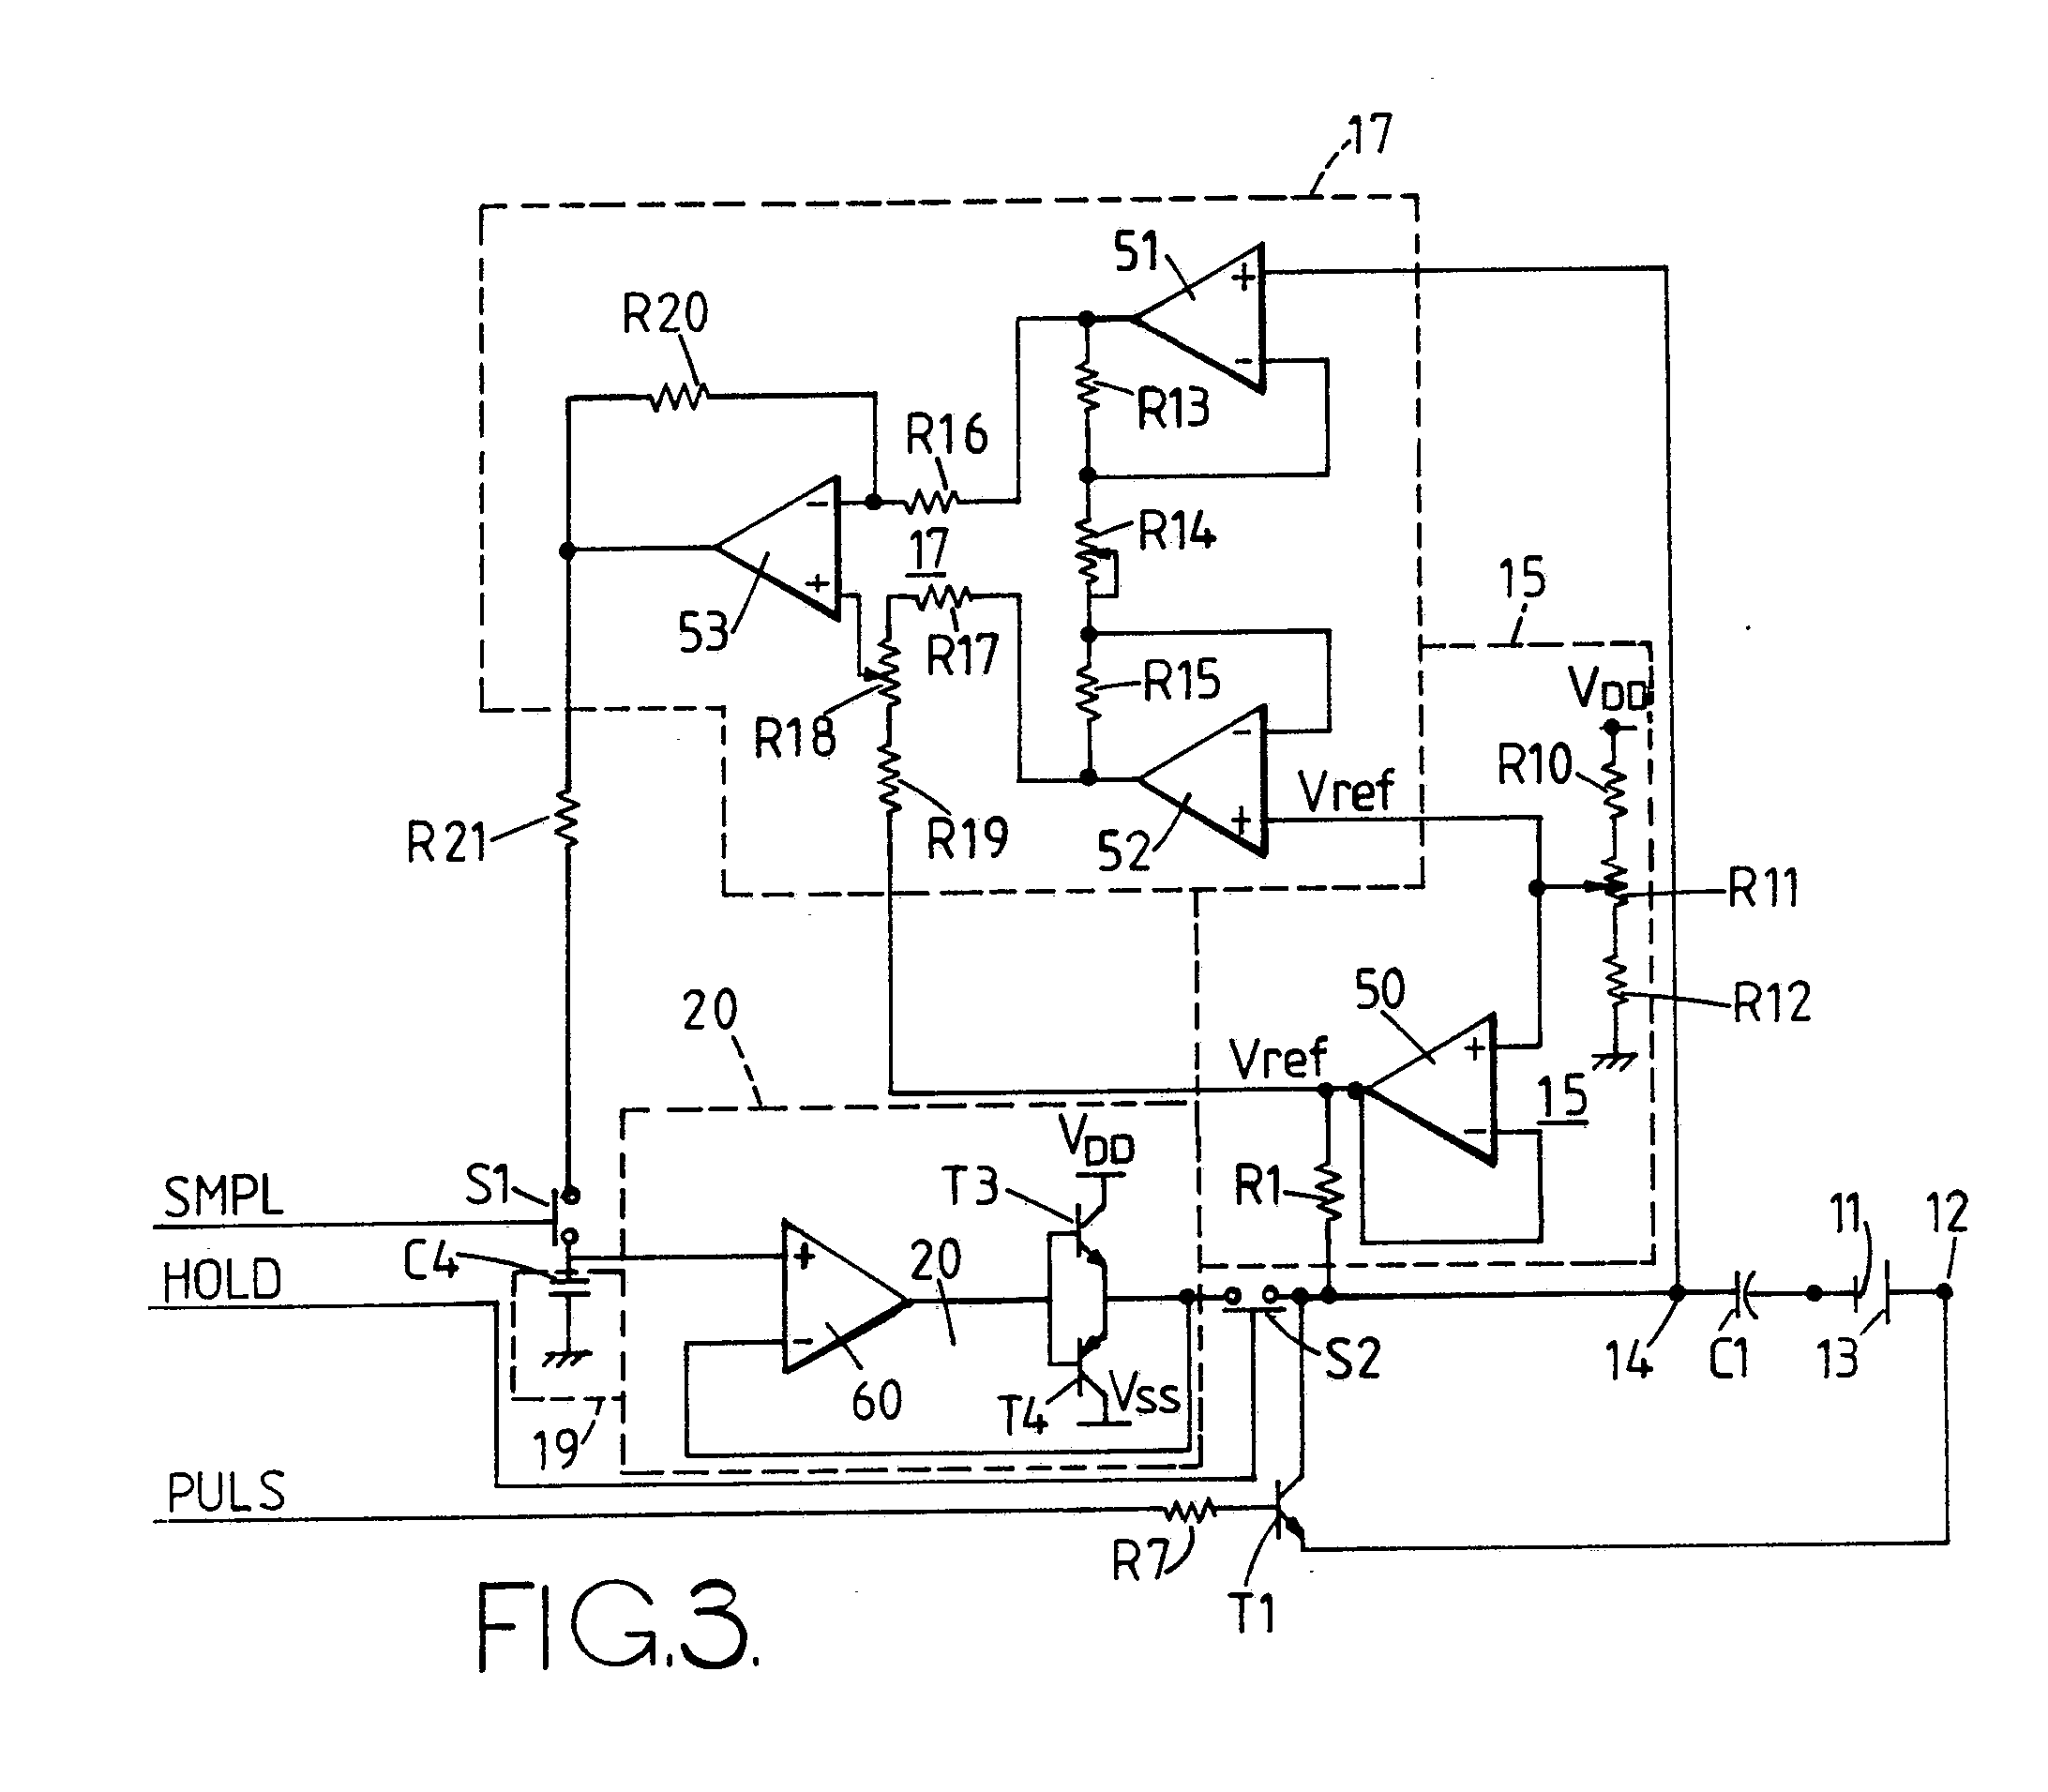
\includegraphics[width=9.9cm]{./bilder/PacemakerCircuit.png}
\end{textblock*}

\vissteduatt{Visste du att .... något mer om kth medtech eller BME? ELLER visste du att Pacemakern är en Lundauppfinning?}


\newpage


\subsection*{Mer jul} 
\index[alfa]{Mer jul}
\index[anfa]{Mer jul} 
\songinfo{Av: Falk Adolphson
}

\begin{parse lines}[\noindent]{#1\\}
    Jag är en lugn person med takt och ton
    måttfull och balanserad
    Jag är tyst och still och det ska mycket till 
    innan jag blir exalterad
    Men jag har en last som håller mig fast 
    i ett järngrepp varje vinter
    När året är slut och snön ligger djup 
    och slädarnas medar slinter

    Jag vill ha mer jul
    Ge mig mer jul
    Jag vill ha mer jul
    Ge mig mer jul
    Tusen stjärnor som tindrar,
    glitter så långt jag ser
    Av juleljus som glimmar,
    vill jag ha mer


\end{parse lines}

\newpage

\begin{parse lines}[\noindent]{#1\\}
    En show glöms bort om den bara visar opp 
    effekter som man knappast anar
    Så ge mig trettio grader kallt, tomtar överallt 
    och en skog av gröna granar
    Jag vill ha snötyngda hus, tusentals ljus, 
    kulörta kulor i drivor
    Bjällerklang som ackompanjemang 
    på alla julens skivor

    Jag vill ha mer jul…

    Ge mig en svårknäckt nöt, sötare gröt, 
    djupare dopp i grytan
    Glittrigare glim och grötigare rim 
    och mer Arne Weise i rutan
    Jag vill ha rymligare säck, segare knäck, 
    fetare fläsk från grisen
    Krimsigare krams, längre långdans 
    och raskare räv på isen

    Jag vill ha mer jul…

    Jag vill ha mer, mer
    Ge mig mer, mer
    Jag vill ha mer, mer
    Ge mig mer, mer

\end{parse lines}

\vissteduatt{Visste du att Mer Jul spelas årligen i Edekvata oavbrutet från och \\med Glöggillet fram till Julgillet är hållet?}

\newpage

\subsection*{Jag är liten nolla} 
\index[alfa]{Jag är liten nolla}
\index[anfa]{Jag är liten nolla}
\songinfo{Mel: Jag är fattig bonddräng\\
Text: JO Sivtoft, E94}

\begin{parse lines}[\noindent]{#1\\}
    Jag, en liten nolla, på Elektro jag går
    Dagar går och kommer, medan jag pluggar på
    Labbar, löddar, räknar, programmerar och lär, 
    Går på föreläsning, inför tentan jag svär

    Jag en fattig nolla, pasta lever jag på
    Och när fredan kommer till Edekvata jag gå
    Sen, när jag blitt livad, vill jag dansa, umgås
    Vila hos en flicka, vill jag också förstås

    Sen så kommer helgen, och då vill CSN
    Att jag pluggar satan, men då festar jag än
    40 timmars vecka, gäller inte för oss
    För oss teknologer, e de dubbelt förstås

    Så går hela veckan, varje läsperiod
    Åren går och kommer, men jag är vid gott mod
    Jag tar mina tentor, samlar på mig poäng, 
    Jag tar min examen, sen så blir jag utslängd

    Nu så väntar livet, som civilingenjör
    Nu så ska jag skörda, tjäna pengar som smör
    Men man jobbar sliter, si så där 40 år
    Till barn, familj o staten, alla pengarna går

    Så när dagen kommer, invid himmelens port, 
    Lite rädd och lessen, för de synder jag gjort
    Inte skattefuska, köra fort, supa loss
    Herren Gud i himlen, är väl missnöjd förstas

    Jag, vid pärleporten, blir nu eftertänksam
    De allra bästa åren, alltför snabbt de försvann
    Hade allt för bråttom, bort från de som var bäst
    Åren på Elektro, saknar jag allra mest

    Men då säger Herren: (civil) ingenjören, kom hit! 
    Jag har sett din strävan, och ditt eviga slit
    Därför, ingenjören, är du välkommen här
    Himmelens Elektro till du antagen är

    Jag som liten ängel, står så still inför Gud, 
    och sen klär han på mej en Elektrovit skrud
    Nu du, säger Herren, börjar vi om igen 
    Nu du, liten nolla, nu har du kommit hem

    Till dig liten nolla, sensmoralen den är
    Ha ej allt för bråttom, under tiden du lär
    Tids nog får du jobba, resten utav ditt liv
    Därför ta till vara, på studentlivets tid
\end{parse lines}

\vissteduatt{Visste du att... sjunges gärna på nollegasque(???)}


\newpage

\subsection*{Hacke Hackspett} 
\index[alfa]{Hacke Hackspett}
\index[anfa]{Hacke Hackspett}
\songinfo{Mel: Woody Woodpecker (Georg F. Tibbles, Ramey Idriss)\\
Text: Povel Ramel \& Georg Eliasson
}

\begin{parse lines}[\noindent]{#1\\}
     %\textit{Mitt namn är Hacke Hackspett, resande i Schweizerostar!}
    Hahahahaha! Hahahahaha! Hör på hackspettens melodi
    Hahahahaha! Hahahahaha! Med sin hackande harmoni!
    
    Han hackar sig fram
    ifrån stam till stam
    och bygger upp sitt höga C
    När du märker hans skratt,
    så ta på dig din hatt
    ty han är på jakt efter tre
    
    ||: Hahahahaha! Hahahahaha! 
    Har du hört en så’n retfull trall,
    Hahahahaha! Hahahahaha! 
    När du traskar bland gran och tall
    
    Om hans skönsång nu ej
    gör nå't intryck på dig,
    alla hackspettars hjärtan slår
    
    Hahahahaha! Hahahahaha! Varje gång det är sol och vår :||
\end{parse lines}

\vissteduatt{Visste du att Povel Ramel och hans glättiga gröngölingar spelade in\\
 låten på 78-varvare 23 september 1948?}


\newpage


\input{kapitel/03-andra_sektioner.tex}

\input{kapitel/04-klassiska_visor.tex}

\input{kapitel/05-skånska_visor.tex}

\begin{center}
    \vspace*{1.5cm}
    {\fontsize{20}{20}\textbf{Teknologvisor}}\\
    \vspace{0.7cm}
    {\fontsize{12}{12}\textit{Om teknologen själv får välja}}
\end{center}
\addtocwithheader{Teknologvisor}  % Add entry to TOC and set header\noBackground
\noBackground

\newpage
\resetBackground


\subsection*{Porthos visa} 
\index[alfa]{Porthos visa}
\index[anfa]{Jag vill börja gasqua!}
\songinfo{Mel: You can't get a man with a gun \\(ur Annie get your gun)\\Text: T Andrén}
\colorbox{yellow}{Vi måste bestämma hur texten ska vara. Samma som i förra boken \\eller ska vi följa vad vi hittar i andra böcker eller online?}

\begin{parse lines}[\noindent]{#1\\}
    Jag vill börja gasqua!
    Var fan är min flaska?
    Vem i helvete stal min butelj?
    Skall mej törsten betvinga?
    En TT börja svinga?
    Nej för fan bara blunda och svälj!
    Vilken smörja!
    Får jag spörja?
    Vem för fan tror att jag är en älg?
    Till England vi rider,
    och sedan vad det lider,
    träffar vi välan på någon PUB
    Och där skall vi festa!
    Blott dricka utav det bästa
    utav Whiskey och Portvin
    Jag tänker gå hårt in
    för att prova på rubb och stubb
    Rubb och stubb…
\end{parse lines}

\vissteduatt{Visste du att om den sista "stubb" sjunges så måste låten upprepas...}

% \newpage


\subsection*{En komplex värld} 
\index[alfa]{En komplex värld}
\index[anfa]{Alla jävla bevis}
\songinfo{Mel: En helt ny värld (ur Aladdin)\\
Text: Ellinor Persson F07 och Andreas Tågerud F06
}

\begin{parse lines}[\noindent]{#1\\}
    Alla jävla bevis
    inses lätt som en övning.
    Javakursen en prövning
    för min bristande logik.

    Ska man komma ihåg
    alla formler i huvet?
    Formelsamlingen, du vet,
    säger inget om det här!

    En komplex värld
    Vad fan betyder bijektiv?
    Ingenting stämmer här, där allt jag lär,
    blir glömt snart efter tentan.
    Hur ska det gå?
    Och det är bara vecka två...
    Känner en underton av aggression
    mot allt Sven Spanne skrivit i sin bok

    (Jag kan transponera den...)
\end{parse lines}

\newpage

\begin{parse lines}[\noindent]{#1\\}
    Jag kan lära dig C
    Matematiska under
    Oförglömliga stunder
    när vi tentar mekanik

    Det ska nog gå!
    Det sa din mamma med igår
    All tid tillvaratas, jag är i fas,
    och bor i mattehuset.
    Nu är jag lärd!
    Till denna svåra ekvation
    jag på frekvenssidan en lösning fann,
    den låg där i en helt ny värld: Laplace!
\end{parse lines}

\subsection*{Enhetsvisan / SI - Système International d'Unités} 
\index[alfa]{Enhetsvisan / SI - Système International d'Unités}
\index[anfa]{1, 2, 75, 6, 7}
\songinfo{Mel: Studentsången}

\begin{parse lines}[\noindent]{#1\\}
    W kg m Wb s
    Ω m T A rad
    cd Sv N s
    Ω A m lx dB
    °C W/m²
    J/kg H V C
    kg/m3 mol
    m/s²
    m/s²
    F !
\end{parse lines}

\vissteduatt{Visste du att SI-låttexten finns i TeFyma?}

\newpage

\subsection*{Man ska ha matlab} 
\index[alfa]{Man ska ha matlab}
\index[anfa]{Man ska ha matlab}
\songinfo{Mel: Man ska ha husvagn}

\begin{parse lines}[\noindent]{#1\\}
    Jag har prövat nästan allt som finns att pröva på
    Beta, kulram, räknesticka, tärning eller så
    Jag har kalkylerat på de konstigaste sätt
    och nu så har jag kommit på hur man ska räkna rätt

    Man ska ha MATLAB - då är kalkylen redan klar
    Man ska ha MATLAB - det har jag sett att andra har
    Man ska ha MATLAB - det är min livsfilosofi
    Man ska ha MATLAB - för då blir man fri

    I många år så var jag inte alls så särskilt lärd
    Jag visste ej vad som vänta' mig i denna stora värld
    Men sen kom jag till LTH, och ända sedan dess
    så har jag funnit livets stora lyxdelikatess

    Man ska ha MATLAB - så man slipper tänka alls
    Man ska ha MATLAB - ja, då går allting som en vals
    Man ska ha MATLAB - det bygger på nån slags logik
    Man ska ha MATLAB - för då blir man rik

    5 minuter mekanik och 5 minuter statfys
    5 minuter plottande och 5 minuter analys
    5 minuter fråga phadder, 5 minuter stopp
    5 minuter tänka själv och sen så ger man opp
\end{parse lines}

\vissteduatt{Vad kom först MATLAB eller Maple?}

\newpage

\begin{parse lines}[\noindent]{#1\\}
    Man ska ha MATLAB - och datasalens friska luft
    Man ska ha MATLAB - det tycker tjejerna är tufft
    Man ska ha MATLAB - när ryssen kommer med sitt MIG
    Man ska ha MATLAB - då vinner man i krig!
\end{parse lines}

\vissteduatt{visste du att}

\newpage

\subsection*{Teknologvisa} 
\index[alfa]{Teknologvisa}
\index[anfa]{Jag är teknolog och helt OK}
\songinfo{Mel: The Lumberjack Song (Monty Python)\\ Sångarstriden 1982\\ Kursivt sjunges av sångförman}

\noindent\textit{Jag är teknolog och helt OK\\
Jag jobbar hårt och jag roar mig}\\\\
\noindent Han är teknolog och helt OK\\
Han jobbar hårt och han roar sig\\\\
\noindent\textit{Teknik är ball\\
Jag kan Pascal\\
Till Lophtet vill jag gå\\
Där träffas alla vänner\\
som är från LTH}\\\\
\noindent Teknik är ball\\
Han kan Pascal\\
Till Lophtet vill han gå\\
Där träffas alla vänner\\
som är från LTH\\\\
\noindent För han är teknolog och helt OK\\
Han jobbar hårt och han roar sig\\\\

\vissteduatt{Visste du att "Han" kan eneklt bytas ut mot "Hon" eller "Hen"!}

\newpage

\noindent\textit{Min mattebok \\
den gör mig klok\\
Jag läser kärnfysik\\
Jag går på föreläsning\\
och älskar juridik}\\\\
\noindent Hans mattebok\\
den gör han klok\\
Han läser kärnfysik\\
Han går på föreläsning\\
och älskar juridik???\\\\
\noindent Men han är teknolog och helt OK\\
Han jobbar hårt och han roar sig\\\\
\noindent\textit{Som ekonom jag blir fantom\\
Konkurser gör mig säll\\
Till flickor blankt jag nekar\\
Jag älskar en tabell}\\\\
\noindent Som ekonom han blir fantom???\\
konkurser...\\
Nää, BUU!!\\\\
\noindent Men han är teknolog och helt OK\\
Han jobbar hårt och han roar sig\\


\newpage

\subsection*{Flerdimensionell ångest} 
\index[alfa]{Flerdimensionell ångest}
\index[anfa]{Flerdimensionell ångest}
\songinfo{Mel: Härjarevisan\\
Text: Daniel Milve F11}

\begin{parse lines}[\noindent]{#1\\}
    Jag har aldrig sett mig själv som välkalkylerad
    Riktningsderivata gör min hjärna punkterad
    Man borde börjat lyssna redan
    Typ när nollningen tog stopp
    Än har jag ingen aning om vad Green’s formel säger
    Dock vet jag klart och tydligt vad de dryga förtäljer:
    Skillnaden mellan kurs och fest är 
    Kurser kan man göra om!

    Men så nu ska vi ut och tenta
    Statens små bidrag hämta
    Differentialer, integral och vektoranalys (i planet!)
    Fem timmar med hårda tag och
    Nu änteligen lär jag
    Kunna dra nån nytta av vad Månsson sade vecka två!
\end{parse lines}

\vissteduatt{Visste du att...}


\newpage


\subsection*{O, hemska labb} 
\index[alfa]{O, hemska labb}
\index[anfa]{O, hemska labb}
\songinfo{Mel: O, helga natt}

\colorbox{orange}{OSÄKER PÅ DENNA}

\begin{parse lines}[\noindent]{#1\\}
    O, hemska labb, o grymma kval imorgon
    Här sitter jag och förstår ingenting
    Hela mitt inre är fyllt utav ett motstånd
    emot eländig elektrisk mätteknik
    Jag skulle nog behöva lite ledning,
    här räcker inte min kapacitans
    Kondensatorer och felvända dioder
    O, hemska labb nu vill jag koppla af
    O, hemska labb ty detta blir min graf

    O, hemska labb, o grymma kval imorgon
    Här sitter jag och förstår ingenting
    Hela programmet är fyllt utav funktioner
    som innehåller en himla massa fel
    Pekare som inte har nån riktning,
    oändliga loopar, oj vad jag blir sträng!
    Åh, kompilera, hur ska det här fungera?
    O, hemska labb, nu vill jag logga ut
    O, hemska labb, ty detta blir mitt slut
\end{parse lines}

\vissteduatt{Visste du att...}


\newpage


\subsection*{Tenta efter jul} 
\index[alfa]{Tenta efter jul}
\index[anfa]{Tenta efter jul}
\songinfo{Mel: Mössens julafton\\
Skriva om att D-sektionen vinnande bordvisa (SåS enligt sångarkiv)}

\colorbox{yellow}{OSÄKER PÅ DENNA}

\begin{parse lines}[\noindent]{#1\\}
    När julen börjar närmas
    och man vill koppla av
    Så kommer tentaplugget
    här och ställer sina krav

    Jag börjar kompromissa
    gör julrimmen i C
    Försöker strukturera
    pluggar fram till klockan tre

    Programmering lin-jär algebra
    Endim å reglerteknik är ingenting att ha
    Tenta efter nyår är ju trist
    Men skippar man för många ja då blir man alkolist

    Skål! 
\end{parse lines}

\vissteduatt{Visste du att...}


\newpage




\input{kapitel/07-ölvisor.tex}

\begin{center}
    \vspace*{1.5cm}
    {\fontsize{20}{20}\textbf{Vinvisor}}\\
    \vspace{0.7cm}
    {\fontsize{12}{12}\textit{Om den nytvättade vita skjortan själv får välja}}
\end{center}
\addtocwithheader{Vinvisor}  % Add entry to TOC and set header\noBackground
\noBackground

\newpage
\resetBackground

\subsection*{\colorbox{red}{Tar bort: Lovsången till kvinnan}} 
% \index[alfa]{Öl, öl, öl i glas}
% \index[anfa]{Öl, öl, öl i glas}
% \songinfo{Mel: Row your boat}

\begin{parse lines}[\noindent]{#1\\}
    tas bort
\end{parse lines}

\vissteduatt{Visste du att...}

\newpage

\subsection*{Feta fransyskor} 
\index[alfa]{Feta fransyskor}
\index[anfa]{Feta fransyskor}
\songinfo{Mel: Militärmarsch av Schubert\\
K-sektionen Sångarstriden 1985}

\begin{parse lines}[\noindent]{#1\\}
    Feta fransyskor som svettas om fötterna,
    de trampar druvor
    som sedan ska jäsas till vin
    Transpirationen viktig é,
    ty den ge'
    fin bouquet
    Vårtor och svampar följer me'
    men vad gör väl de'?

    För vi vill ha vin,
    vill ha vin,
    vill ha mera vin,
    även om följderna blir
    att vi må lida pin
    Flaskan och glaset gått i sin
    Hit med vin, mera vin!
    Tror ni att vi är fyllesvin?
    {\Large Ja!} (Fast större!)
\end{parse lines}

\vissteduatt{Visste du att...}


\newpage


\subsection*{Lyft ditt välförsedda glas} 
\index[alfa]{Lyft ditt välförsedda glas}
\index[anfa]{Lyft ditt välförsedda glas}
\songinfo{Mel: Ding dong merrily on high}

\begin{parse lines}[\noindent]{#1\\}
    Lyft ditt välförsedda glas
    Det är en härlig börda
    Nu har grabbarna kalas
    Ve segern snart skall skörda
    //: Ding dingedingeding dingedingeding
    dingedingeding dong dong
    Imorgon är det lördag ://

    Sätt nu glaset till din mun
    Se döden på dig väntar
    Nu har grabbarna kalas
    Hör liemannen flämtar
    //: Ding dingedingeding dingedingeding
    dingedingeding dong dong
    Begravningsklockor klämtar ://
\end{parse lines}

\vissteduatt{Visste du att...}


\newpage


\subsection*{Bordeaux, bordeaux} 
\index[alfa]{Bordeaux, bordeaux}
\index[anfa]{Jag minns än idag hur min fader}
\songinfo{Mel: I sommarens soliga dagar}

\begin{parse lines}[\noindent]{#1\\}
    Jag minns än idag hur min fader
    kom hem ifrån staden så glader
    och rada' upp flaskor i rader
    och sade nöjd som så:
    "Bordeaux, Bordeaux!"

    Han drack ett glas, kom i extas,
    och sedan blev det stort kalas
    Och vi små glin, ja vi drack vin
    som första klassens fyllesvin
    Och vi dansade runt där på borden
    och skrek så vi blev blå:
    "Bordeaux, Bordeaux!"
\end{parse lines}

\vissteduatt{Visste du att...}


\newpage


\subsection*{Vinbröder} 
\index[alfa]{Vinbröder}
\index[anfa]{Två bröder, Jan-Ove och Hadar}
\songinfo{Mel: I sommarens soliga dagar}

\begin{parse lines}[\noindent]{#1\\}
    Två bröder, Jan-Ove och Hadar,
    de plockade fram sina spadar,
    och grävde en grop bakom huset.
    De hade en idé:
    Vaddå, vaddå?
    Jo, priset på 
    Kir och Bordeaux,
    är högt men om man gjorde så,
    att man i gropen lade ner,
    två kilo jäst och en back MER,
    så skulle det nog vara möjligt
    att producera vin i detta hål! Skål!
\end{parse lines}

\vissteduatt{Visste du att...}


\newpage


\subsection*{Karnaugh, karnaugh} 
\index[alfa]{Karnaugh, karnaugh}
\index[anfa]{Karnaugh, karnaugh}
\songinfo{Mel: I sommarens soliga dagar}

\begin{parse lines}[\noindent]{#1\\}
    Jag minns än i dag hur min fader
    kom hem i från labbet så glader
    och rada' upp bitar i rader
    och sade glad som så:
    Karnaugh, Karnaugh!

    Å ett å noll \& noll å ett 
    å booleska uttryck det är fett!
    Med ett å noll \& noll å ett,
    ska du nu se att det blir rätt,
    Men vi felsökte våra signaler,
    och det blev fel ändå
    Karnaugh, Karnaugh!
\end{parse lines}

\vissteduatt{Visste du att...}


\newpage


\subsection*{I sommarens soliga dagar} 
\index[alfa]{I sommarens soliga dagar}
\index[anfa]{I sommarens soliga dagar}
\songinfo{Mel: I sommarens soliga dagar\\
Text: Anders Nilsson $\pi$03 och Björn Carlin $\pi$02}

\begin{parse lines}[\noindent]{#1\\}
    I sommarens soliga dagar
    Kall rå fisk till alla vi lagar
    Och sätter oss ute i hagar
    Där maten härsken står
    Bakteriehärd av solen närd
    Den höjer högt sitt blanka svärd
    Men mot dess hot vi funnit bot 
    Vi sätter spritens krafter mot
    För spriten kan döda det mesta
    Vi hälsan återfår, Gutår! Gutår!
\end{parse lines}

\vissteduatt{Visste du att...}


\newpage


\subsection*{Kosmetisk visa} 
\index[alfa]{Kosmetisk visa}
\index[anfa]{Du behöver inte ha nåt läppstift alls}
\songinfo{Mel: She’ll be Coming ‘Round the Mountain\\
Lundakarnevalen 2002}

\begin{parse lines}[\noindent]{#1\\}
    Du behöver inte ha nåt läppstift alls,
    du behöver inte ha nåt läppstift alls,
    för när vinet börjar flöda,
    färgas läpparna ju röda,
    liksom tungan, hakan, skjortan och din hals!
\end{parse lines}

\vissteduatt{Visste du att...}


\newpage


\subsection*{Magnumflaskan Åkesson} 
\index[alfa]{Magnumflaskan Åkesson}
\index[anfa]{Magnumflaskan Åkesson}
\songinfo{Mel: Teddybjörnen Fredriksson\\
Lundakarnevalen 2010}

\begin{parse lines}[\noindent]{#1\\}
    För längesen, när jag fyllde 15 år
    fick jag en flaska av min mor
    Hon sa "Mitt barn, dela den med vännerna
    För den är faktiskt ganska stor."

    Magnumflaskan Åkesson,
    du var så stor och tung
    Jag gick runt med dig i hand,
    och i Dalby var jag kung

    Magnumflaskan Åkesson,
    din kork försvann i skyn
    Men jag drack dig bara själv
    Och kräktes i hela byn
\end{parse lines}

\vissteduatt{Visste du att...}


\newpage


\subsection*{\colorbox{orange}{Korkskruvens visa}} 
% \index[alfa]{Magnumflaskan Åkesson}
% \index[anfa]{Magnumflaskan Åkesson}
\songinfo{Mel: Nu har vi ljus}

\begin{parse lines}[\noindent]{#1\\}
    TA BORT???

    Nu har vi rus här i vårt hus
    Korken är borta hopptralalala
    Doften är ljuv, jag är en skruv,
    jag är en skruv.

    Jag kan inte öppna bag-in-boxen,
    jag kan inte öppna bag-in-boxen

    Lalalala lalalala lalalalala lala
\end{parse lines}

\vissteduatt{Visste du att...}


\newpage


\subsection*{Dance macabre} 
\index[alfa]{Dance macabre}
\index[anfa]{runt våran stuga, små djävlar sluga}
\songinfo{Mel: Vårvindar friska}

\begin{parse lines}[\noindent]{#1\\}
    Runt våran stuga, små djävlar sluga
    tassa så tyst med bockfot och svans
    Varulvar yla, isande kyla
    sveper i dimman, fantygets dans
    Bäva, o broder, lyssna och hör
    vrålen från gast, som osalig dör
    Satan han skrattar,
    flaskan han fattar,
    super tills dagen gryr.

    Gastar och spöken
    skymta i köken,
    dödingar släpa ruttnande lik
    Benrangel skramla,
    spökhänder famla,
    kväva din strupes rosslande skrik
    Helvetes alla fasor släpps loss
    Fan rider här med hela sin tross
    Göm dig i stugan,
    du har fått flugan
    Dille det blir din lott

\end{parse lines}

\vissteduatt{Visste du att man viskar hela låten fram till \\ "Helvetets alla fasor..." då tar man i för Kung och fosterland?}


\newpage




\newpage
\resetBackground
\printindex[alfa]
\printindex[anfa]
\newpage

\end{document}
